\section{Neural Networks and Deep Learning}



\subsection[Neural networks]{Neural Networks in Keras}




\begin{frame}{Neural Networks}
	\begin{itemize}
		\item In ``classical'' machine learning, we predict an outcome directly based on the input features
		\item In neural networks, we can have ``hidden layers'' that we predict
		\item These layers are not necessarily interpretable
		\item ``Neurons'' that ``fire'' based on an ``activation function''
	\end{itemize}
	
\end{frame}


\begin{frame}[standout]
Note that in our earlier example with our EmbeddingVectorizer, we essentially added a ``layer'' between the input and the output. Now, we generalize this idea.

\end{frame}

\begin{frame}
	
	\def\layersep{2.5cm}
	
	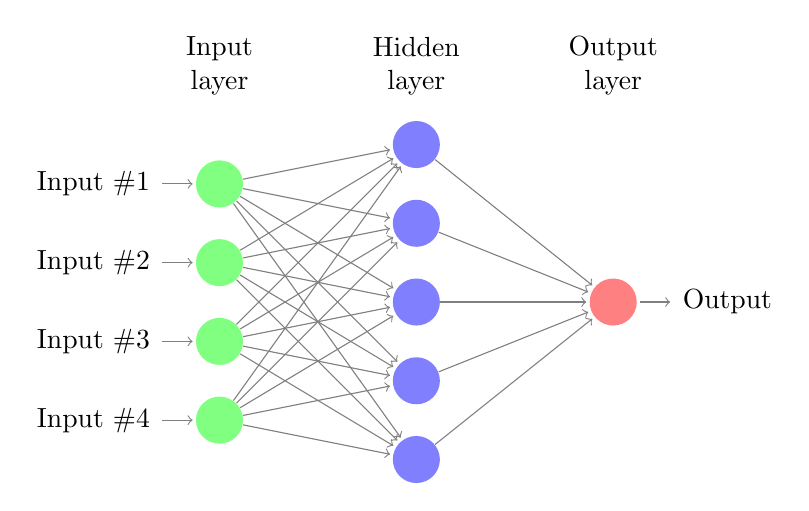
\begin{tikzpicture}[shorten >=1pt,->,draw=black!50, node distance=\layersep]
	\tikzstyle{every pin edge}=[<-,shorten <=1pt]
	\tikzstyle{neuron}=[circle,fill=black!25,minimum size=17pt,inner sep=0pt]
	\tikzstyle{input neuron}=[neuron, fill=green!50];
	\tikzstyle{output neuron}=[neuron, fill=red!50];
	\tikzstyle{hidden neuron}=[neuron, fill=blue!50];
	\tikzstyle{annot} = [text width=4em, text centered]
	
	% Draw the input layer nodes
	\foreach \name / \y in {1,...,4}
	% This is the same as writing \foreach \name / \y in {1/1,2/2,3/3,4/4}
	\node[input neuron, pin=left:Input \#\y] (I-\name) at (0,-\y) {};
	
	% Draw the hidden layer nodes
	\foreach \name / \y in {1,...,5}
	\path[yshift=0.5cm]
	node[hidden neuron] (H-\name) at (\layersep,-\y cm) {};
	
	
	% Draw the output layer node
	\node[output neuron,pin={[pin edge={->}]right:Output}, right of=H-3] (O) {};
	
	% Connect every node in the input layer with every node in the
	% hidden layer.
	\foreach \source in {1,...,4}
	\foreach \dest in {1,...,5}
	\path (I-\source) edge (H-\dest);
	
	% Connect every node in the hidden layer with the output layer
	\foreach \source in {1,...,5}
	\path (H-\source) edge (O);
	
	% Annotate the layers
	\node[annot,above of=H-1, node distance=1cm] (hl) {Hidden layer};
	\node[annot,left of=hl] {Input layer};
	\node[annot,right of=hl] {Output layer};
	\end{tikzpicture}
	
	$\Rightarrow$ If we had multiple hidden layers in a row, we'd call it a \emph{deep} network.
\end{frame}




\begin{frame}{Why neural networks?}
  \begin{itemize}
  \item learn hidden structures (e.g., embeddings (!))
  \item go beyond the idea that there is a direct relationship between occurrence of word X and label (or occurrence of pixel [R,G,B] and a label)
  \item images, machine translation --- and more and more general NLP, sentiment analysis, etc.
  \end{itemize}
  
  \small {Example of a comparatively easy introduction:
    \url{https://towardsdatascience.com/neural-network-embeddings-explained-4d028e6f0526}}

\end{frame}


\begin{frame}[fragile]{Simple feed forward network}
\begin{lstlisting}
model.add(Dense(300, input_dim=input_dim, activation='relu'))
model.add(Dense(1, activation='sigmoid'))
\end{lstlisting}	
	
\begin{itemize}[<+->]
\item Our first layer reduces the input features (e.g., the 10,000 features our CountVectorizer creates) to 300 neurons
\item It does so using the relu function $f(x) = max(0, x)$ (as our counts cannot be negartive, just a linear function)
\item The second layer reduces the 300 neurons to 1 output neuron using the sigmoid function (the S curve you know from logistic regression)
\item Of course, we can add multiple layers in between if we want to
\end{itemize}
\end{frame}





\begin{frame}{Convolutional networks}
  The problem with such a basic networks: just as with classic SML, we still loose all information about order (the ``not good'' problem).
  Therefore,
  \begin{itemize}
  \item We concatenate the vectors of neighboring words
  \item We apply some filter (essentially, we detect patterns)
  \item and then pool the results (e.g., taking the maximum)
  \end{itemize}
  This means that we now excplitly take into acount \emph{the temporal structure} of a sentence.
\end{frame}



\begin{frame}{Convolutional networks}
  \makebox[\columnwidth]{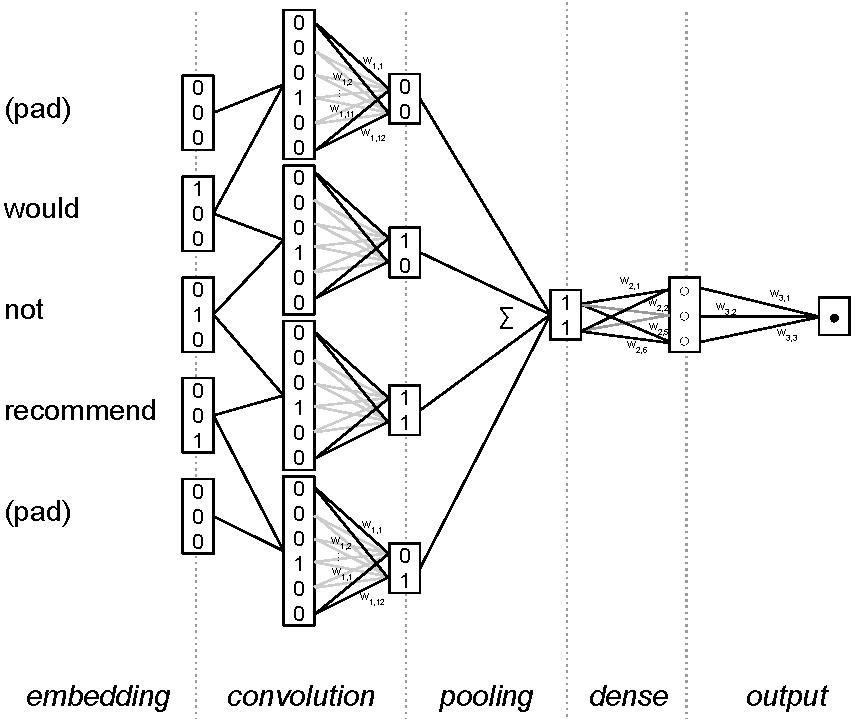
\includegraphics[width=\columnwidth,height=.8\paperheight,keepaspectratio]{ch09_cnn_cropped}}
\end{frame}



\begin{frame}[fragile]{Convolutional networks}
\begin{lstlisting}
model.add(Embedding(input_dim=vocab_size, output_dim=embedding_dim, input_length=maxlen))
model.add(Conv1D(embedding_dim, 5, activation='relu'))
model.add(GlobalMaxPooling1D())
model.add(Dense(300, activation='relu'))
model.add(Dense(1, activation='sigmoid'))
\end{lstlisting}	
The layers:	
\begin{enumerate}[<+->]
\item train an embedding model
\item apply the convolution with 5 ``timestamps''
\item pool using the maximum
\item another layer with 300 dimensions
\item the final layer with 1 output neuron
\end{enumerate}
\end{frame}


\begin{frame}{Convolutional networks}
  \textbf{Note that the preprocessing differs!}
  
  \begin{itemize}
  \item We do not take a word vector per document as input any more, but \emph{a sequence of words}
  \item For concatenating, these sequences need to have equal length, which is why we \emph{pad} then
  \end{itemize}
	
\end{frame}




\begin{frame}{LSTM (long short-term memory)}
  \begin{itemize}
  \item Unlike ``feed forward'' neural networks, this is  a ``recurrent neural network'' (RNN) -- the training works in two directions
  \item Heavy in computation, very useful for predicting \emph{sequences}
  \item Won't cover today
  \end{itemize}
\end{frame}




\begin{frame}{The embedding layer}
  \begin{itemize}
  \item Often, the first layer is creating word embeddings
  \item Good embeddings need a lot of training data
  \item Training good embeddings needs time
  \item Therefore, we can replace that layer with a pre-trained embedding layer (!)
  \item We can even use a hybrid approach and allow the pre-trained embedding layer to be re-trained!
  \end{itemize}
\end{frame}



\begin{frame}[standout]
  There are example notebooks on github!
\end{frame}
